% !TEX root = ../../main.tex
\section{Natural selection (survival of the fittest)}
1859 marked the year that Charles Darwin shocked the world with the incredible
insights contained in his book \textit{On the origin of Species}. The complete 
title of the book \textit{On the Origin of Species by Means of Natural
Selection, or the Preservation of Favoured Races in the Struggle for Life}
pretty well captures Darwin's proposed mechanism for how evolution takes place.
Nowadays with the so-called modern-synthesis of evolution we know that natural
selection is not the only evolutionary force that shapes living organisms. In
the coming sections we will mathematically explore mechanisms such as mutation
and genetic drift that all contribute to form the many \textit{endless forms,
most beautiful} that live in our planet. But we will begin with the first
evolutionary force discovered by Darwin and Alfred Russel Wallace.

Natural selection is intrinsically associated with the concept of fitness. The
frase "survival of the fittest" first used by Darwin guided and still guides
the way that biologists think about the evolution of many organisms. But
despite the fact that fitness is part of the daily jargon of many biologists,
it is a subtle and highly debated concept. After all what defines the ability
of an organism to survive the challenges that suround them are completely
context depdendet. Roughly speaking we can think of fitness as the ability of
an organism, or a population of organisms to survive and reproduce in the given
ecological niche they occupy. The term ecology has to be included because
fitness is a result of the interplay between organisms with their environment
including all biotic and abiotic interactions. 

It is common both in theory and in experiments to use the relative growth rates
of organisms, i.e. the speed at which they can reproduce and generate
offspring, as a proxy for scientists. This is a convenient approximation both
for experiments and for theory, but one should not lose track of the imperant
context dependence on the fitness. Just because redwoods have an average life
span of 500-700 years and a very low growth rate that doesn't mean they are not
fit. Having said that we will first begin with the simplest form of fitness,
i.e. frequency independent selection. The term frequency independence simply
refers to the assumption that the fitness of a particular allele does not
depend on the relative abundance of such allele. This assumption could break
down for cases such as some pathogenic bacteria that coordinate their attack
via cell-to-cell communication known as quorum sensing. But we need to learn
how to crawl before we try to run.

\subsubsection{Frequency independent selection (haploids)}

Because of our personal love for bacteria and the fact that many of the most
interesting experiments in evolution have been and are being done in haploid
organisms, we will first focus our efforts on these single-cell organisms.
Haploidy refers to the biological feature of having a single copy of a
chromosome. As bacteria divide into two cells they segregate (split) one copy
of the genome to each of the daughter cells (extrachromosomal elements such as
plasmids behave differently). This in contrast with diploidy where organisms
such as humans that receive one copy of each chromosome form each parent. What
haploidy means for our task of modeling selection on a one-locus two-allele
system is that we only need to focus on the fitness value of each of the
alleles without having to worry about combination of alleles.

For the simplest case of one-locus two-alleles let us define the two alleles to
be $A$ and $a$. Let $N_A(t)$ and $N_a(t)$ be the corresponding number of
organisms carrying each allele at time $t$. For the frequency-independent 
selection we have that the change in number of organisms with allele $A$ is of
the form
\begin{equation}
  \dt{N_A} = f_a N_A(t),
\end{equation}
where $f_a$ is the growth rate of organisms carrying this allele on a
particular fixed environment. As discussed before we will use this growing rate
as a proxy for fitness; this is sometimes called Malthusian fitness after
Thomas Robert Malthus, a famous scholar whose assay on population growth
inspired boyh Darwin and Wallace. We can define an equivalent equation for
allele $a$ with fitness $f_a$.

We are not particularly interested in tracking the absolute number of organisms
with a specific genotype, but their relative abundance. Therefore let us define
$N\tot(t) \equiv N_A(t) + N_a(t)$ and the relative abundance of allele $A$ as
\begin{equation}
  x(t) = {N_A(t) \over N\tot(t)}.
\end{equation}
The time dynamics for $N\tot(t)$ are of the form
\begin{equation}
  \dt{N\tot(t)} = \bar{f}(t) N\tot(t),
\end{equation}
where $\bar{f}(t)$ is the average fitness of the population at time $t$. We can
deduce its value if we notice that the dynamics of the total population is just
the sum of the individual alleles dynamics, i.e.
\begin{equation}
  \dt{N\tot(t)} = \dt{N_A(t)} + \dt{N_a(t)} = f_a N_A(t) + f_a N_a(t).
\end{equation}
We can factorize an $N\tot(t)$ out of the equation and use the frequencies of
each allele to obtain
\begin{equation}
  \dt{N\tot(t)} = N\tot(t) \left[ f_a x(t) + f_a (1 - x(t)) \right].
\end{equation}
This shows us that the average fitness $\bar{f}$ is of the form
\begin{equation}
  \bar{f}(t) = f_a x(t) + f_a (1 - x(t)).
\end{equation}

The dynamics that interest us are the dynamics of the allele frequency. We only
need to define the dynamics for one of the alleles since we are assuming a
two-allele model for which knowing the dynamics of one of them determines the
dynamics of the other. This looks like
\begin{equation}
  \dt{x} = \dt{}\left( {N_A(t) \over N\tot(t)} \right).
\end{equation}
Using the chain rule this gives
\begin{equation}
  \dt{x(t)} = {\dot{N}_A(t) N\tot(t) - N_A(t) \dot{N}\tot(t) \over N\tot(t)^2},
\end{equation}
where $\dot{N}_x = dN_x / dt$. Substituting the time derivatives gives
\begin{equation}
  \dt{x} = {[f_a N_A(t)] N\tot(t) \over N\tot(t)^2} -
           {N_A(t)[\bar{f}(t) N\tot(t)] \over N\tot(t)^2}.
\end{equation}
We now substitute the defintion of the average fitness to obtain
\begin{equation}
  \dt{x} = {f_a N_A(t) - 
           N_A(t) [f_a x(t) + f_a (1 - x(t))]
          \over N\tot(t)},
\end{equation}
This can be further simplify by using the definition of the allele frequency to
obtain
\begin{equation}
  \dt{x} f_a x(t) - x(t)[f_a x(t) + f_a (1 - x(t))].
\end{equation}
Grouping terms by the fitness values results in
\begin{equation}
  \dt{x} = f_a x(t)(1 - x(t)) - f_a x(t)(1 - x(t))
  = s x(t)(1 - x(t)),
  \label{eq_freq_dynamics_selection}
\end{equation}
where we defined $s = f_a - f_a$, the fitness difference between both alleles,
also known as the selection coefficient. This differential equation is very
revealing; what it is telling us is that for there to be changes in the
population structure, i.e. for the population to evolve there needs to be a
fitness difference between the competing members of the population. For now
ignore that we are working under the unrealistic regime of unbounded
exponential growth, meaning that as the model is written, there is no upper
bound for how large a population could get. The central feature of
\eref{eq_freq_dynamics_selection} is that for there to be a change in the
composition of the population, which is what we define as evolution, the
fitness values for each mutant must differ. 

For the specific case that we are studying in which $s$ is a constant, meaning
that the fitness values of the alleles don't change over time we can solve this
differential equation. Specifically we can use the separation of variables
method to compute
\begin{equation}
  \int {dx \over x(1 - x)} = \int dt \;s,
  \label{eq_sep_var}
\end{equation}
where we drop thte time dependence for notation convenience. For the left-hand
side of the equation we can use partial fractions and write
\begin{equation}
  {1 \over x(1 - x)} = {A \over x} + {B \over (1 - x)}
  = {A - Ax + Bx \over x(1 - x)}.
\end{equation}
For $A = 1$ and $B = 1$ we have
\begin{equation}
  {1 - x + x \over x(1 - x)} = {1 \over x(1 - x)}.
\end{equation}
This allows us to write \eref{eq_sep_var} as 
\begin{equation}
  \int {dx \over x} + \int {dx \over 1 - x} = s \int dt.
\end{equation}
Solving these integrals results in
\begin{equation}
  \ln x - \ln(1 - x) = \ln\left( {x \over 1 - x} \right) 
  = s t + C,
  \label{eq_sep_var_sol}
\end{equation}
where $C$ is an integration constant. If we set an initial condition $x(t = 0)
= x_o$ we find that
\begin{equation}
  C = \ln \left( {x_o \over 1 - x_o} \right).
\end{equation}
Substituting this value for $C$ and exponentiating both sides of
\eref{eq_sep_var_sol} gives
\begin{equation}
  {x \over 1 - x} = {x_o \over 1 - x_o} \E^{s t}
\end{equation}
Let's now solve for $x$. First we send the denominator on the left-hand side to
the other side
\begin{equation}
  x = (1 - x)\left( x_o \over 1 - x_o \right)\E^{st}
\end{equation}
Now we expand the product and send the terms with $x$ back to the left-hand
side
\begin{equation}
  x + x {x_o \over 1 - x_o}\E^{st} = {x_o \over 1 - x_o}\E^{st}.
\end{equation}
Factorizing $x$ resutls in
\begin{equation}
  x \left( 1 + {x_o \over 1 - x_o}\E^{st} \right) = {x_o \over 1 - x_o}\E^{st}.
\end{equation}
The term in parenthesis can be rewritten as
\begin{equation}
  x \left( {1 - x_o + x_o\E^{st} \over 1 - x_o} \right) =
  {x_o \over 1 - x_o}\E^{st}.
\end{equation}
This allows us to cancel the denominator on both sides of the equation to
obtain
\begin{equation}
  x \left[ 1 + x_o \left( \E^{st} - 1 \right) \right] = x_o \E^{st}.
\end{equation}
Finally we can solve for the allele frequency
\begin{equation}
  x = {x_o \E^{st} \over 1 + x_o \left( \E^{st} - 1 \right)}.
\end{equation}
This is the solution of the logistic equation. \fref{fig01_01} shows this
solution for different selection coefficients.

\begin{figure}[h!]
	\centering 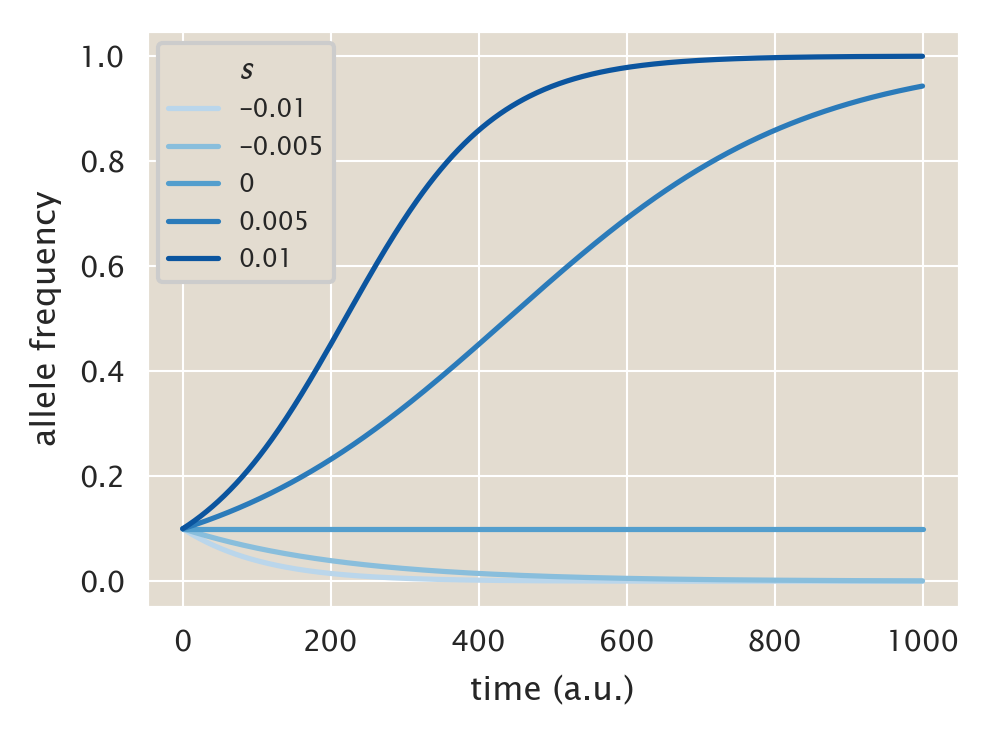
\includegraphics
  {../fig/deterministic_evo/01_01_deterministic_select.png}
  \caption{\textbf{Allele frequency for deterministic selection}. The 
	different cuves show allele frequency dynamics for a one-locus two-allele
	system. The fate of the allele is determined by the value of the selection
	coefficient, but the speed to fixation depends both on the initial allele
	frequency and on the magnitude of the selection coefficient.}
  \label{fig01_01}
\end{figure}